\documentclass{beamer}
\usepackage{tut}

\def\tuttitle{Prolog}
\date{2016-12-12/13}

\prolog

\begin{document}
\normalsize
\normalem

\begin{frame}[plain]
  \titlepage
\end{frame}

\begin{frame}
  \frametitle{Vier Farben}
  Nach dem Vier-Farben-Satz kann jede beliebige Landkarte mit nur vier Farben so gefärbt werden,
  dass keine zwei aneinandergrenzenden Gebiete die gleiche Farbe bekommen.
  In dieser Aufgabe soll eine solche Belegung für die Telefonvorwahlbereiche in Deutschland gefunden werden.
  \begin{figure}
    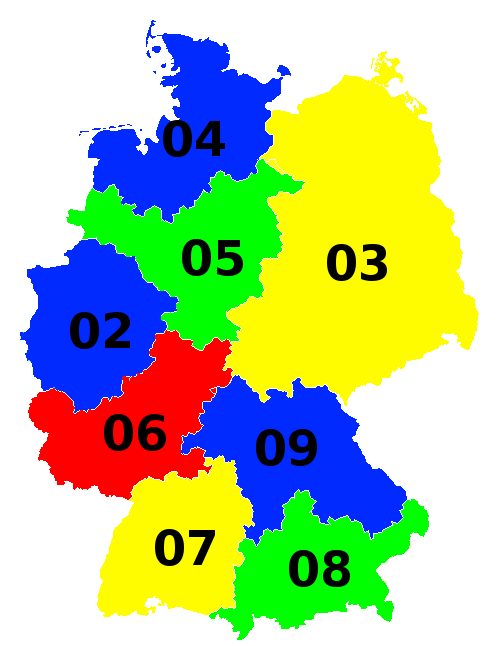
\includegraphics[height=0.5\textheight]{tut7-deutschland}
  \end{figure}
\end{frame}

\begin{frame}[fragile]
  \frametitle{Vier Farben}
  Definiere Prädikat \lstinline{farbe}, welches die vier zu verwendenden Farben festlegt.
  \pause
  \begin{lstlisting}
    farbe(gruen).
    farbe(gelb).
    farbe(blau).
    farbe(rot).
  \end{lstlisting}
  (In SWI-Prolog kann man auch Umlaute verwenden.)
\end{frame}

\begin{frame}[fragile]
  \frametitle{Vier Farben}
  Definiere Prädikat \lstinline{nachbar(X,Y)}, welches erfüllt ist,
  wenn Länder der Farben \lstinline{X} und \lstinline{Y} Nachbarn sein dürfen,
  d.\,h., wenn \lstinline{X} und \lstinline{Y} unterschiedliche Farben sind.
  (Hinweis: wir wollen uns später eine Lösung \emph{generieren} lassen,
  also muss das Prädikat auch für uninstanziierte Variablen funktionieren.)
  \pause
  \begin{lstlisting}
    nachbar(X, Y) :- farbe(X), farbe(Y), X \= Y.
  \end{lstlisting}
\end{frame}

\begin{frame}[fragile]
  Definiere Prädikat \lstinline{deutschland},
  welches Topologie der Karte der 8~Vorwahlbereiche in Deutschland beschreibt.
  \begin{figure}
    \begin{subfigure}{0.3\textwidth}
      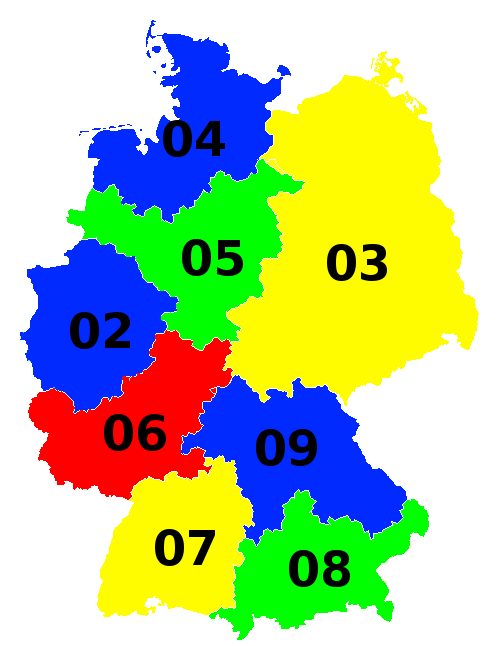
\includegraphics[height=0.5\textheight]{tut7-deutschland}
    \end{subfigure}
    \pause
    \begin{subfigure}{0.65\textwidth}
      \begin{lstlisting}
        deutschland(
          V2, V3, V4, V5,
          V6, V7, V8, V9) :-
         nachbar(V2,V5), nachbar(V2,V6),
         nachbar(V3,V4), nachbar(V3,V5),
           nachbar(V3,V6), nachbar(V3,V9),
         nachbar(V4,V5),
         nachbar(V5,V6),
         nachbar(V6,V7), nachbar(V6,V9),
         nachbar(V7,V8), nachbar(V7,V9),
         nachbar(V8,V9).
      \end{lstlisting}
    \end{subfigure}
  \end{figure}
\end{frame}

\begin{frame}[fragile]
  \frametitle{Vier Farben}
  Wie erhält man nun gültige Einfärbung der Karte?
  \pause
  \begin{lstlisting}
    ?- deutschland(V2,V3,V4,V5,V6,V7,V8,V9).
    V2 = V3, V3 = V7, V7 = gruen,
    V4 = V6, V6 = V8, V8 = blau,
    V5 = V9, V9 = gelb .
  \end{lstlisting}
\end{frame}

\begin{frame}
  \frametitle{Vier Farben}
  Wie findet man heraus, ob die Karte auch nur mit drei Farben färbbar ist?
  
  \pause
  Einen der \lstinline{farbe}-Fakten entfernen und Anfrage erneut stellen.
  
  \pause
  Alternativ: feststellen, dass auch mit vier \lstinline{farbe}-Fakten eine Lösung mit nur drei Farben herauskam.
\end{frame}

\begin{frame}
  \frametitle{Tester, Generatoren, Ausführungsbäume}
  Die Prädikate \lstinline{odd} und \lstinline{even} sind in zwei Varianten gegeben:
  \lstinputlisting[caption=Tester]{tut7-tester.pl}
  \lstinputlisting[caption=Generatoren]{tut7-generatoren.pl}
\end{frame}

\begin{frame}
  \frametitle{Tester, Generatoren, Ausführungsbäume}
  \lstinputlisting{tut7-tester.pl}
  Warum können die Tester nicht als Generatoren verwendet werden?
  
  \pause
  \lstinline{?even(X)} findet zwar zunächst \lstinline{X=0},
  danach schlagen aber die Teilziele \lstinline{X>0} und \lstinline{X1 is X-1} für \emph{uninstanziiertes} \lstinline{X} fehl –
  arithmetische Operationen und \lstinline{is} sind nur für instanziierte Variablen zugelassen.
\end{frame}

\begin{frame}
  \frametitle{Tester, Generatoren, Ausführungsbäume}
  \lstinputlisting{tut7-generatoren.pl}
  Warum können die Generatoren nicht als Tester verwendet werden?
  
  \pause
  Erfüllbare Anfragen, z.\,B. \lstinline{?even(2)}, funktionieren zunächst.
  Bei Reerfüllung und bei nicht erfüllbaren Anfragen (z.\,B. \lstinline{?even(3)}) versucht Prolog aber,
  mit immer größeren \lstinline{Y} die Bedingung \lstinline{X is Y+1} zu erfüllen,
  ohne erkennen zu können, dass es nie funktionieren wird.
\end{frame}

\begin{frame}
  \frametitle{Tester, Generatoren, Ausführungsbäume}
  \lstinputlisting{tut7-generatoren.pl}
  Was passiert, wenn bei den Generatoren die Teilziele \lstinline{X>1} und \lstinline{X>0} weggelassen werden?
  
  \begin{description}
  \pause
  \item[\texttt{X>1}]
    \lstinline{odd(1)} kann nun sowohl direkt als auch über \lstinline{even(0)} gezeigt werden,
    \lstinline{?odd(X)} generiert daher die 1 doppelt.
    Jede andere Zahl über 1, ob gerade oder ungerade, wird letztlich auf \lstinline{odd(1)} zurückgeführt und damit ebenfalls doppelt generiert.
  \pause
  \item[\texttt{X>0}]
    Keine Auswirkung.
    Alle an dieser Stelle erreichten Zahlen sind als Nachfolger einer ungeraden Zahl bereits $>1>0$.
  \end{description}
\end{frame}

\begin{frame}
  \frametitle{Tester, Generatoren, Ausführungsbäume}
  \lstinputlisting{tut7-generatoren.pl}
  Im Folgenden (Aufgabenblatt + Tafel) sind für die Anfrage \lstinline{?even(X)} die Ausführungsbäume zum Zeitpunkt der Ausgabe von \lstinline{X=0} und \lstinline{X=2} dargestellt.
  Zeichne Ausführungsbaum zum Zeitpunkt der Ausgabe von \lstinline{X=4}; welches Teilziel schlägt dabei einmal fehl?
\end{frame}

\begin{frame}
  \frametitle{Wolf, Ziege, Kohl}
  Das klassische Wolf-Ziege-Kohl-Rätsel.
  In Prolog lässt sich die Situation als 4-Tupel \lstinline{(Mann,Ziege,Wolf,Kohl)} von Ufern darstellen,
  z.\,B.~\lstinline{(rechts,links,links,rechts)}.
\end{frame}

\begin{frame}[fragile]
  \frametitle{Wolf, Ziege, Kohl}
  Definiere einstelligen Tester \lstinline{erlaubt(Situation)},
  der genau für Situationen erfüllt ist, in denen keines der Dinge gefressen wird.
  
  \pause
  Zur Ausnutzung von Symmetrie:
  \begin{lstlisting}
    gegenueber(links,rechts).
    gegenueber(rechts,links).
  \end{lstlisting}
  \pause
  \begin{lstlisting}
    erlaubt((Mann,Ziege,_,_)) :- Mann = Ziege.
    erlaubt((_,Ziege,Wolf,Kohl)) :-
      gegenueber(Ziege,Wolf),
      gegenueber(Ziege,Kohl).
  \end{lstlisting}
  
  (\lstinline{_} ist wie in Haskell eine „Wegwerf-Variable“
  und kann in \lstinline{(Mann,Ziege,_,_)} für zwei verschiedene Ufer stehen.)
\end{frame}

\begin{frame}[fragile]
  \frametitle{Wolf, Ziege, Kohl}
  Definiere dreistelligen Generator \lstinline{fahrt(S1,F,S2)},
  der zu Situation \lstinline{S1} bei Reerfüllung alle Situationen \lstinline{S2} generiert,
  die durch einfache Flussüberfahrt entstehen können.
  Zeichenkette \lstinline{F} beschreibt dabei die Fahrt, z.\,B. \lstinline{'leer'}, \lstinline{'Ziege'}.
  
  \sout{Geben Sie dabei lediglich die Regeln für Überfahrten mit Ziege, sowie die für leere Fahrten an.}

  \pause
  \begin{lstlisting}
    fahrt((U,Z,W,K), 'leer', (U2,Z,W,K)) :- gegenueber(U,U2).
    fahrt((U,U,W,K), 'Ziege', (U2,U2,W,K)) :- gegenueber(U,U2).
    fahrt((U,Z,U,K), 'Wolf', (U2,Z,U2,K)) :- gegenueber(U,U2).
    fahrt((U,Z,W,U), 'Kohl', (U2,Z,W,U2)) :- gegenueber(U,U2).
  \end{lstlisting}
\end{frame}

\begin{frame}[fragile]
  \frametitle{Wolf, Ziege, Kohl}
  Das Prädikat \lstinline{loesung(Fahrten)} generiert alle Lösungen des Problems:
  \begin{lstlisting}
    loesung(Fahrten) :- start(S), ziel(Z),
                        erreichbar(S,[],Fahrten,Z).
    start((links,links,links,links)).
    ziel((rechts,rechts,rechts,rechts)).
  \end{lstlisting}
  Das dazu benötigte vierstellige Prädikat \lstinline{erreichbar(S,Besucht,Fahrten,Z)}
  ist für Startsituation \lstinline{S} und Zielsituation \lstinline{Z} erfüllt,
  wenn \lstinline{Z} von \lstinline{S} durch Folge von \lstinline{fahrt}en erreichbar ist.
  Es dürfen nur \lstinline{erlaubt}e Zwischensituationen entstehen,
  und um Endlosschleifen zu vermeiden, darf keine der Situationen aus \lstinline{Besucht} erneut vorkommen.
  Die Liste \lstinline{Fahrten} enthält die Beschreibungen der einzelnen \lstinline{fahrt}en in richtiger Reihenfolge.
  
  Hinweis: verwende \lstinline{member} und \lstinline{not} aus Vorlesung.
\end{frame}

\begin{frame}[fragile]
  \frametitle{Wolf, Ziege, Kohl}
  \begin{lstlisting}
    erreichbar(S,_,[],S).
    erreichbar(S,Besucht,[Fahrt|Fahrten],Z) :-
      fahrt(S,Fahrt,S2),
      erlaubt(S2),
      not(member(S2,Besucht)),
      erreichbar(S2,[S2|Besucht],Fahrten,Z).
  \end{lstlisting}
\end{frame}

\begin{frame}[fragile]\lstset{language=Haskell}
  \frametitle{\lstinline{splits}}
  Implementiere Haskell-Funktion
  \begin{lstlisting}
    splits :: [t] -> [([t],[t])]
  \end{lstlisting}
  die alle möglichen Zerlegungen einer Liste in Anfangs- und Endteil berechnet.
  Anfangs- und Endteil werden in Tupel gespeichert,
  Rückgabe ist Liste aller möglichen Tupel.
  \pause
  \begin{lstlisting}
    splits [] = [([],[])]
    splits (x:l) = ([],x:l) : [ (x:s,e) | (s,e) <- splits l ]
  \end{lstlisting}
  \pause
  \begin{lstlisting}
    splits l = [splitAt n l | n <- [0..length l]]
  \end{lstlisting}
\end{frame}

\begin{frame}[fragile]
  \frametitle{\lstinline{splits}}
  Implementiere Prolog-Prädikat
  \begin{lstlisting}
    splits(L, (S,E))
  \end{lstlisting}
  das bei Reerfüllung alle möglichen Zerlegungen von \lstinline{L} in Teile \lstinline{S} und \lstinline{E} liefert.
  
  \pause
  Rekursiv, analog zur ersten Haskell-Version, mit Reerfüllung statt List~Comprehension:
  \begin{lstlisting}
    splits(L, ([],L)).
    splits([X|L], ([X|S],E)) :- splits(L, (S,E)).
  \end{lstlisting}
  
  \pause
  Rückwärtsausführung von \lstinline{append}:
  \begin{lstlisting}
    splits(L, (S,E)) :- append(S, E, L).
  \end{lstlisting}
\end{frame}

\end{document}
